% !TEX root = comparison.tex

\subsection{Comparing Distributions}
\begin{figure*}[htbp] %  figure placement: here, top, bottom, or page
   \centering
   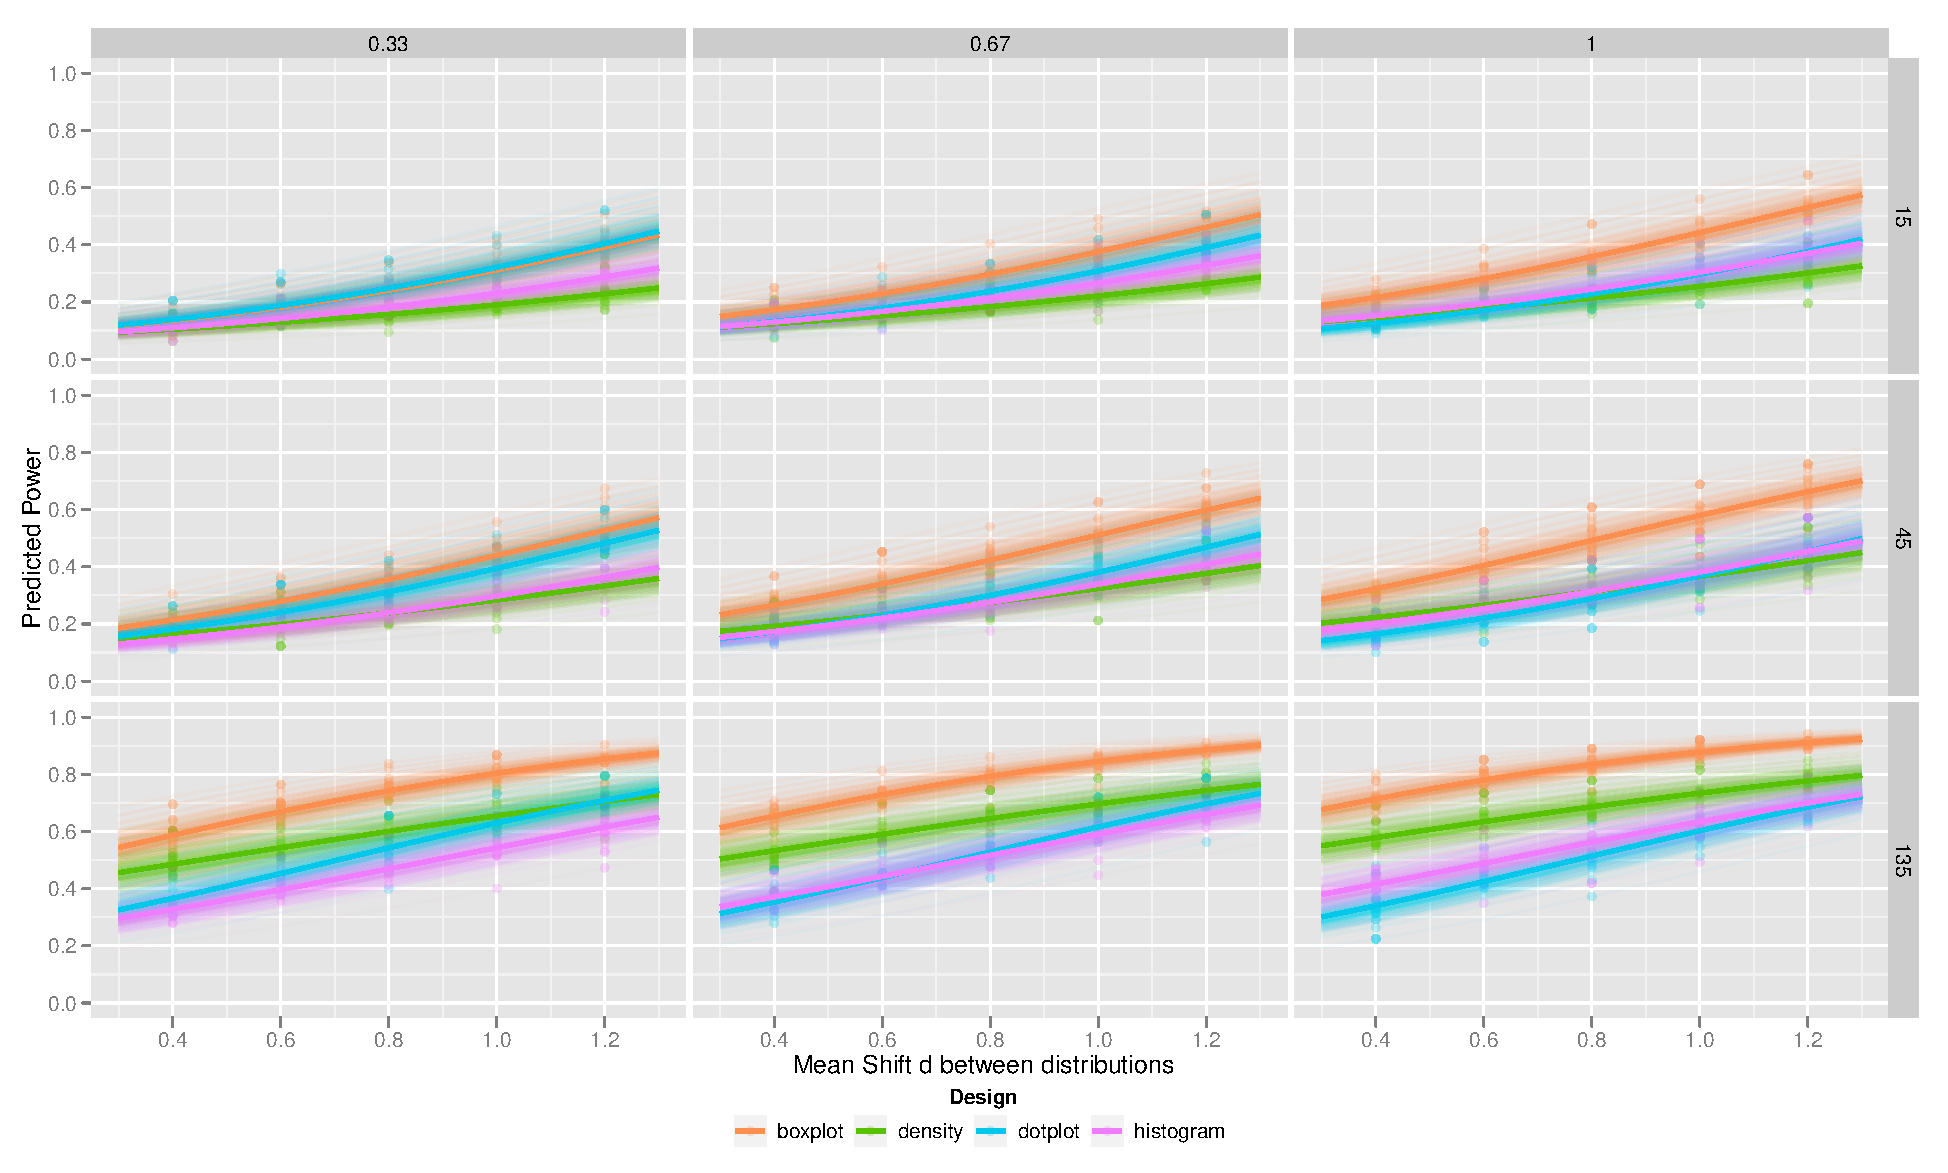
\includegraphics[width=\linewidth]{power-exp2} 
   \caption{Overview of power predictions for the four different designs. The fully saturated thick lines show average predicted power for each of the designs facetted by size of the red group (top to bottom) and relative size of the blue group to the red group (left to right). Thin lines represent variability due to subject-specific abilities. }
   \label{fig:power2}
\end{figure*}

Since each participant provides results from nine lineups, we can use a generalized linear mixed effects model of power and account for individuals' abilities by including a subject-specific random intercept. We included all of the above described covariates  in the model, both as main effects and as two-way interaction with the design to assess their impact on the power of each of the designs.
Figure \ref{fig:power2} summarizes the modeling results as shown in table \ref{tbl:power2}. Generally we can see that the power of all four designs increases with an increase in effect size $d$ (on the $x$ axis), as well as an increasing sample size $n_1$ (top to bottom facetting). Generally, an increase of the second group also is beneficial to power. Unlike all of the other designs,  dotplots actually lose power significantly as the second group increases. 
The reason behind this phenomenon might be visual complexity: dotplots are the only design that show individuals. With an increase in group size, visual complexity increases with it, which could hamper the observer in evaluating shifts.


The two highly summarized designs benefit the most from an increase in sample size: both density charts and boxplots profit significantly more than histograms and dotplots. This might, again, be a hint towards a trade-off between visual complexity and amount of information shown as basis for decisions. 


Table \ref{tbl:speed2} gives an overview of results from a linear model for (log) evaluation time of lineups. Subject-specific speed (due to spatial ability) are accounted for  including a random intercept. Structurally, the model is the same as before, i.e. we regard effect size $d$, size $n_1$ of the first group, and the ratio $n_2/n_1$ between group sizes both as main effects and in two-way interactions with the four competing designs. To make estimate sizes comparable, we have again multiplied all estimates and standard errors involving the group size $n_1$ by 100. This means that we need to interpret those  estimates as average change if the group size is increased by 100 elements. 
The results of this model are similar to the previous: evaluation speeds needed for the four different designs is very close, but  histograms take on average a significantly longer time ($e^{0.23} = 1.26$ seconds) to evaluate than lineups of boxplots. 
Where an increase of sample size led to an increase of accuracy before, we now see that it increases time for evaluation of boxplot slightly, but not significantly so. What is interesting is that evaluation time decreases significantly with an increase in sample size, particularly for dotplots, but also for density charts. This is counter-intuitive to our previous argument on dotplots being affected by visual complexity the most. It seems, that observers of dotplot lineups come to a conclusion faster as sample size increases, albeit more often to  the wrong conclusion. Rather than visual complexity, this might be indicative that over-plotting is problematic in dotplots. While we tried to accommodate for over-plotting by making use of alpha-blending and jittering, this might not have been sufficient for the large sample size.
 
\begin{table}[ht]
\begin{center}
\resizebox{\linewidth}{!} {
\begin{tabular}{lrrrrrl}
  \hline
& & Estimate & Error & $t$-value & \multicolumn{2}{l}{approx $p$-value} \\   \hline
\\[-8pt]
\bf design& Intercept & 3.85 & 0.09 & 42.21 & 0.00 & ***\\ 
&  density & 0.01 & 0.12 & 0.07 & 0.94 \\ 
&  dotplot & 0.03 & 0.12 & 0.26 & 0.80 \\ 
&  histogram & 0.23 & 0.12 & 1.97 & 0.05 & . \\ [2pt]
\multicolumn{2}{l}{\bf covariates}\\
&      d & -0.23 & 0.08 & -3.02 & 0.00 & ***\\ [1pt]
&    n1$_{100}$ & 0.07 & 0.04 & 1.70 & 0.09 & .\\ [1pt]
&  ratio & -0.04 & 0.02 & -1.48 & 0.14  \\ [2pt]
\multicolumn{2}{l}{\bf interactions}\\
&  density:d & 0.11 & 0.11 & 1.02 & 0.31 \\ 
&  dotplot:d & 0.20 & 0.11 & 1.86 & 0.06 & .  \\ 
&  histogram:d & -0.01 & 0.11 & -0.09 & 0.93 \\ [1pt]
&  density:n1$_{100}$ & -0.12 & 0.06 & -2.11 & 0.03 & *\\ 
&  dotplot:n1$_{100}$ & -0.16 & 0.06 & -2.83 & 0.00 & ***\\ 
&  histogram:n1$_{100}$ & -0.05 & 0.06 & -0.93 & 0.35 \\ [1pt]
&  density:ratio & 0.04 & 0.03 & 1.18 & 0.24 \\ 
&  dotplot:ratio & 0.02 & 0.03 & 0.65 & 0.52 \\ 
&  histogram:ratio & 0.00 & 0.04 & 0.04 & 0.97 \\ 
   \hline
\\[-5pt]
   \multicolumn{5}{l}{Signif. codes:  0 `***' 0.001 `**' 0.01 `*' 0.05 `.' 0.1}
\end{tabular}}
\end{center}
\caption{\label{tbl:speed2}Results from a Generalized Linear Mixed Effects Model of (log) time to answer a lineup given design and all two-way interactions with effect size $d$, group size $n_1$, and ratio to second to first group size. Estimate and error for all terms involving $n_1$ are multiplied by a factor of 100 for comparability.
Reference group for all effects are boxplot designs. }
\end{table}

Our third response variable is again the subjective assessment of confidence level. On average participants reported a confidence in their results of  3.41 (on a five point scale with 1=lowest and 5=highest), with a standard deviation of 0.149. Modeling confidence levels with a linear mixed effects model with the same structure as before resulted in only one significant effect beyond the intercept: participants report significantly higher confidence for increased number of  points in dotplot lineups. On average an increase of 100 points leads to an increase in confidence of 0.22 (with a standard error of 0.082). This finding is significant with a $p$-value of 0.007. 
Together with the previous results, we can tell that something worth of further investigation happens in the perception of dotplots as sample sizes increase. 


\begin{figure}[htbp] %  figure placement: here, top, bottom, or page
   \centering
   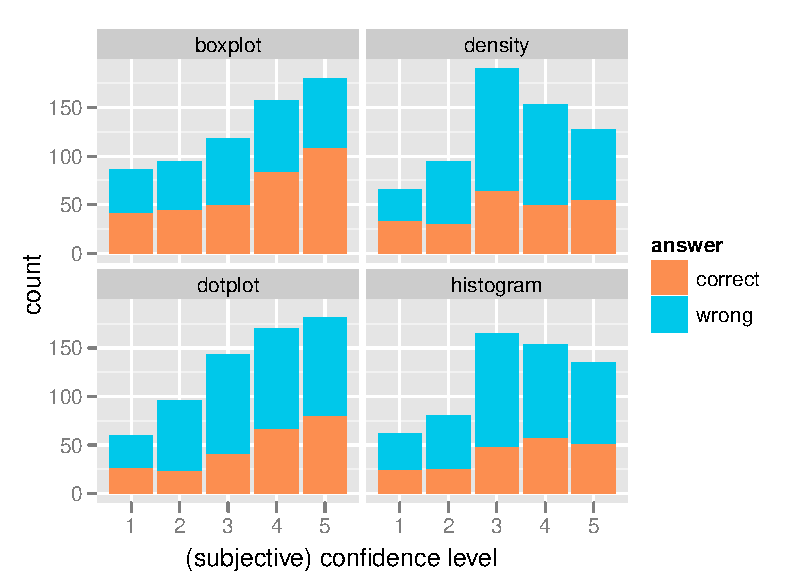
\includegraphics[width=\linewidth]{conf-exp2} 
   \caption{Barcharts of marginal distributions of subjective confidence assessment by design. The distributions display prominent differences.}
   \label{fig:conf-margins}
\end{figure}

Figure \ref{fig:conf-margins} shows barcharts of confidence assessments by design. It is obvious that the distribution of confidence is very different from one design to the next. Boxplots and Dotplots show a similar pattern with an emphasis on high confidence levels, whereas histograms and density lineups have modes at a confidence level of three. One reason behind these differences in confidence distributions might be familiarity with the design - neither density charts nor histograms are particularly frequent displays for a general audience.
